\documentclass{beamer}
\usepackage{ctex}
\usepackage[utf8]{inputenc}
\usepackage{graphicx}
\usepackage{amsmath}
\usepackage{amssymb}
\usepackage{booktabs}
\usepackage{hyperref}
\usepackage{subcaption}
\usepackage{multicol}
\usepackage{listings}
\usepackage{multirow}
\usepackage{tabularx}

\bibliographystyle{alpha}

\usetheme{Madrid}
\usecolortheme{seahorse}

% 自定义块颜色
\setbeamercolor{block title}{bg=blue!30,fg=black}
\setbeamercolor{block body}{bg=blue!10,fg=black}
\setbeamercolor{alertblock title}{bg=red!50,fg=black}
\setbeamercolor{alertblock body}{bg=red!20,fg=black}

% 开启图表编号
\setbeamertemplate{caption}[numbered]

\title{\textbf{周报-向嘉豪(2024年12月10日)}}
\author{向嘉豪}
\institute{衡阳师范学院}
\date{2024年12月10日}

\begin{document}

\begin{frame}
    \titlepage
\end{frame}

\begin{frame}
    \frametitle{摘要}
    \begin{block}{本周主要工作}

        \begin{itemize}
            \item \textbf{论文修订}
           
            \item \textbf{投稿准备}
           
        \end{itemize}
    \end{block}

\end{frame}

\section{论文修订与投稿准备}

\begin{frame}
    \frametitle{论文修订与规范化}
    针对IEEE期刊的格式要求,我们对论文进行了修订,主要包括以下方面:
    \begin{enumerate}
        \item \textbf{符号体系规范化}:
        \begin{itemize}
            \item 引入了\texttt{amssymb}数学符号库,解决了特殊数学符号(如$\ggg$)的显示问题。
            \item 对全文的数学公式和符号进行了统一规范,确保符号使用的一致性和准确性。
        \end{itemize}
        \item \textbf{参考文献完善}:
        \begin{itemize}
            \item 补充了参考文献中缺失的页码范围和期刊卷号等信息。
            
        \end{itemize}
    \end{enumerate}
\end{frame}

\begin{frame}
    \frametitle{投稿准备工作}
    我们按照IEEE计算机学会的出版指南,系统地完成了投稿准备工作:
    \begin{enumerate}
        \item \textbf{熟悉投稿流程}:
        \begin{itemize}
            \item 深入研究了IEEE Author Portal系统(见图\ref{fig:authorportal}),详细了解投稿的每个步骤。
        \end{itemize}
        \item \textbf{撰写投稿信}:
        \begin{itemize}
            \item 按照期刊要求,撰写了投稿信(见图\ref{fig:coverletter}),突出论文的创新性和研究意义。
        \end{itemize}
        \item \textbf{选择合适期刊}:
        \begin{itemize}
            \item 考虑到\textit{IEEE Transactions on Information Forensics and Security}偏重理论研究,经导师指导,决定将论文投向\textit{IEEE Transactions on Computers}。
        \end{itemize}
    \end{enumerate}
\end{frame}

\begin{frame}
    \frametitle{投稿材料}
    \begin{figure}
      \centering
      \begin{subfigure}[b]{0.2\textwidth}
        \centering
        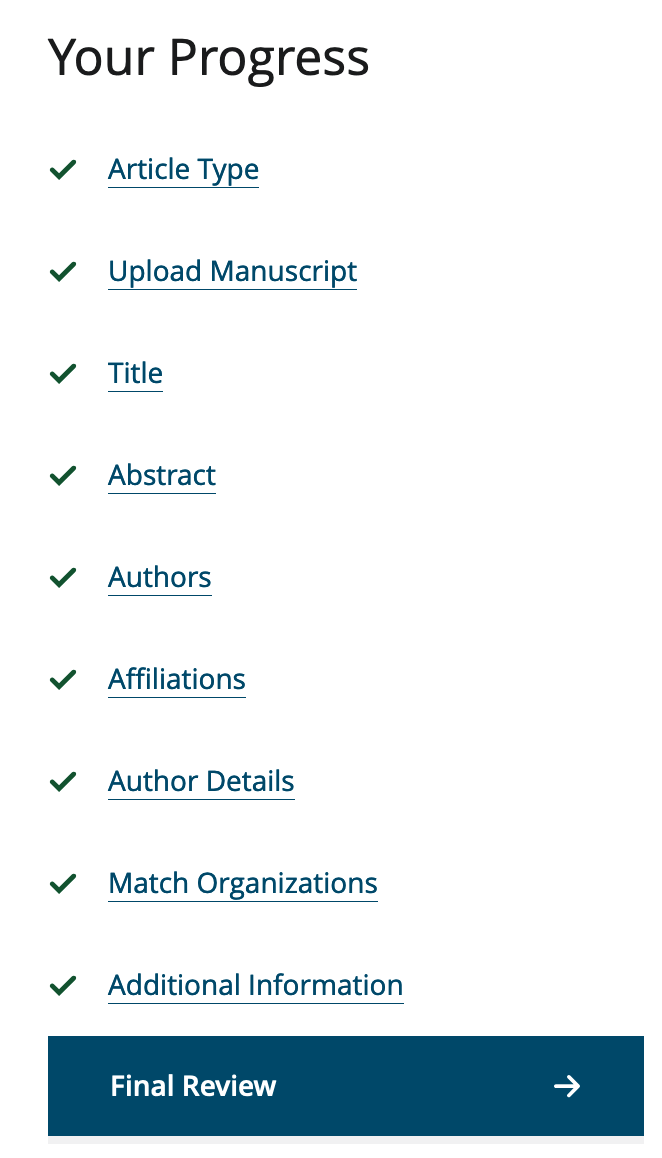
\includegraphics[width=\textwidth]{./fig/submit.png}
        \caption{IEEE Author Portal投稿流程}
        \label{fig:authorportal}
      \end{subfigure}
      \hfill
      \begin{subfigure}[b]{0.45\textwidth}
        \centering
        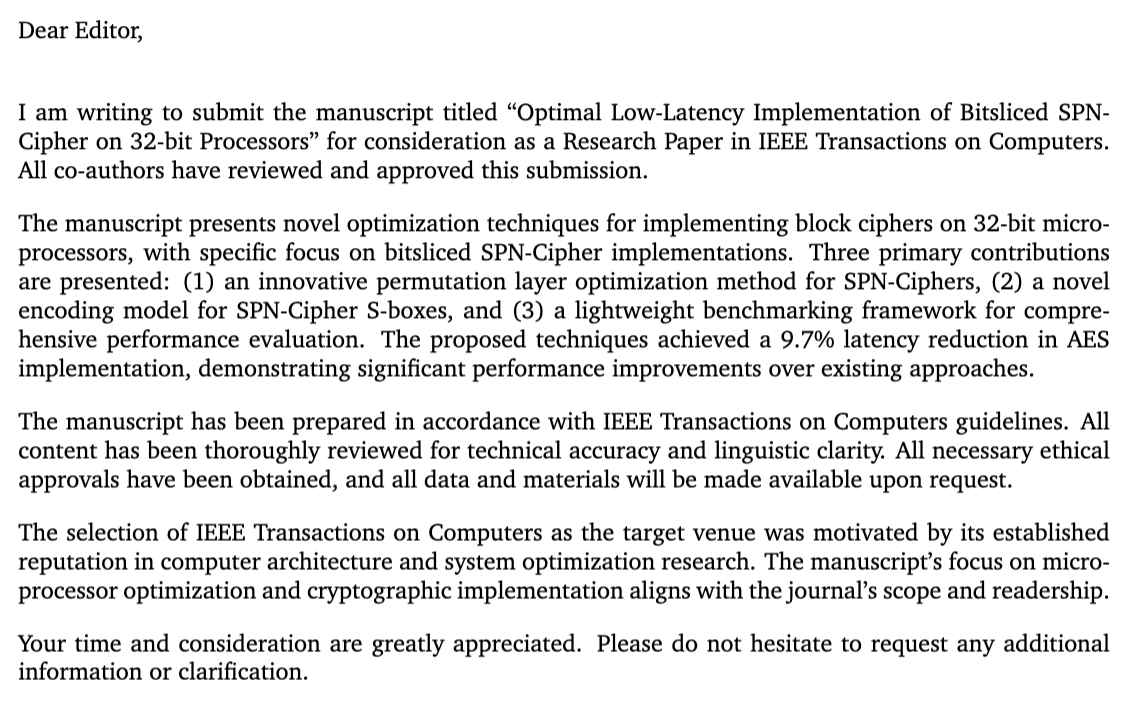
\includegraphics[width=\textwidth]{./fig/CoverLetter.png}
        \caption{投稿信示例}
        \label{fig:coverletter}
      \end{subfigure}
      \caption{论文投稿材料准备}
      \label{fig:submission_materials}
    \end{figure}
\end{frame}

\begin{frame}
    \frametitle{老师评语}
    \begin{alertblock}{去看下拟投稿期刊论文,对自己的论文再提升一下}
      依据该期刊2020年收录《Efficient Software Implementation of Ring-LWE
      Encryption on IoT Processors》软件实现优化论文,对论文进行修改。
  \end{alertblock}
    \begin{block}{本周计划}
      完善论文
    \end{block}
\end{frame}

\end{document}